%   Filename    : chapter_4.tex 
\chapter{Results and Discussions}

\section{Training the Data Set}

Given that the Vehicle Traffic dataset was already preprocessed using Roboflow, it only needs to be trained in YOLOv5 using the available “train.py” file. The following is the code used for the Google Colab Notebook for training the data:


\lstset{language=python,
aboveskip=3mm,
belowskip=3mm,
showstringspaces=false,
columns=flexible,
basicstyle={\small\ttfamily},
numbers=none,
breaklines=true,
breakatwhitespace=true,
tabsize=3
}
\begin{lstlisting}[frame=single]
	!git clone https://github.com/ultralytics/yolov5
	%cd yolov5
	%pip install -qr requirements.txt
	import torch
	import utils
	display = utils.notebook_init()

	
\end{lstlisting}

The data was trained with 16 batches and 300 epochs. These are reflected by the following terminal command for training.


\begin{lstlisting}[frame=single]
		!python /content/yolov5/train.py --batch 16 --epochs 300 --data /content/drive/MyDrive/College/SP/data/data.yaml --weights yolov5m.pt --cache
		
\end{lstlisting}



\newpage

The “/content/drive/MyDrive/College/SP/data/data.yaml” is the yaml file that contains the information about the different classes in the dataset. Below is an example of data.yaml.


\begin{lstlisting}[frame=single]
	
	train: ../train/images
	val: ../valid/images
	test: ../test/images
	
	nc: 6
	names: ['Car', 'Jeepney', 'Motorcycle', 'Tricycle', 'Truck', 'Utility Vehicle']
	
	roboflow:
	workspace: special-project
	project: sp-cmsc198.1
	version: 3
	license: CC BY 4.0
	url: https://universe.roboflow.com/special-project/sp-cmsc198.1/dataset/3
	
	
\end{lstlisting}

The file contains the directory to the train, validation, and testing data as well as other important information such as the number of objects and their names that is needed by”train.py”. 

\section{Results}

Figure \ref{fig:res} shows the statistics of how the data set performed during training.
Notice that as the training progresses the loss values drop. This is the desired behavior as it shows that the training is making fewer mistakes as training continues.


\begin{figure}[h!]
	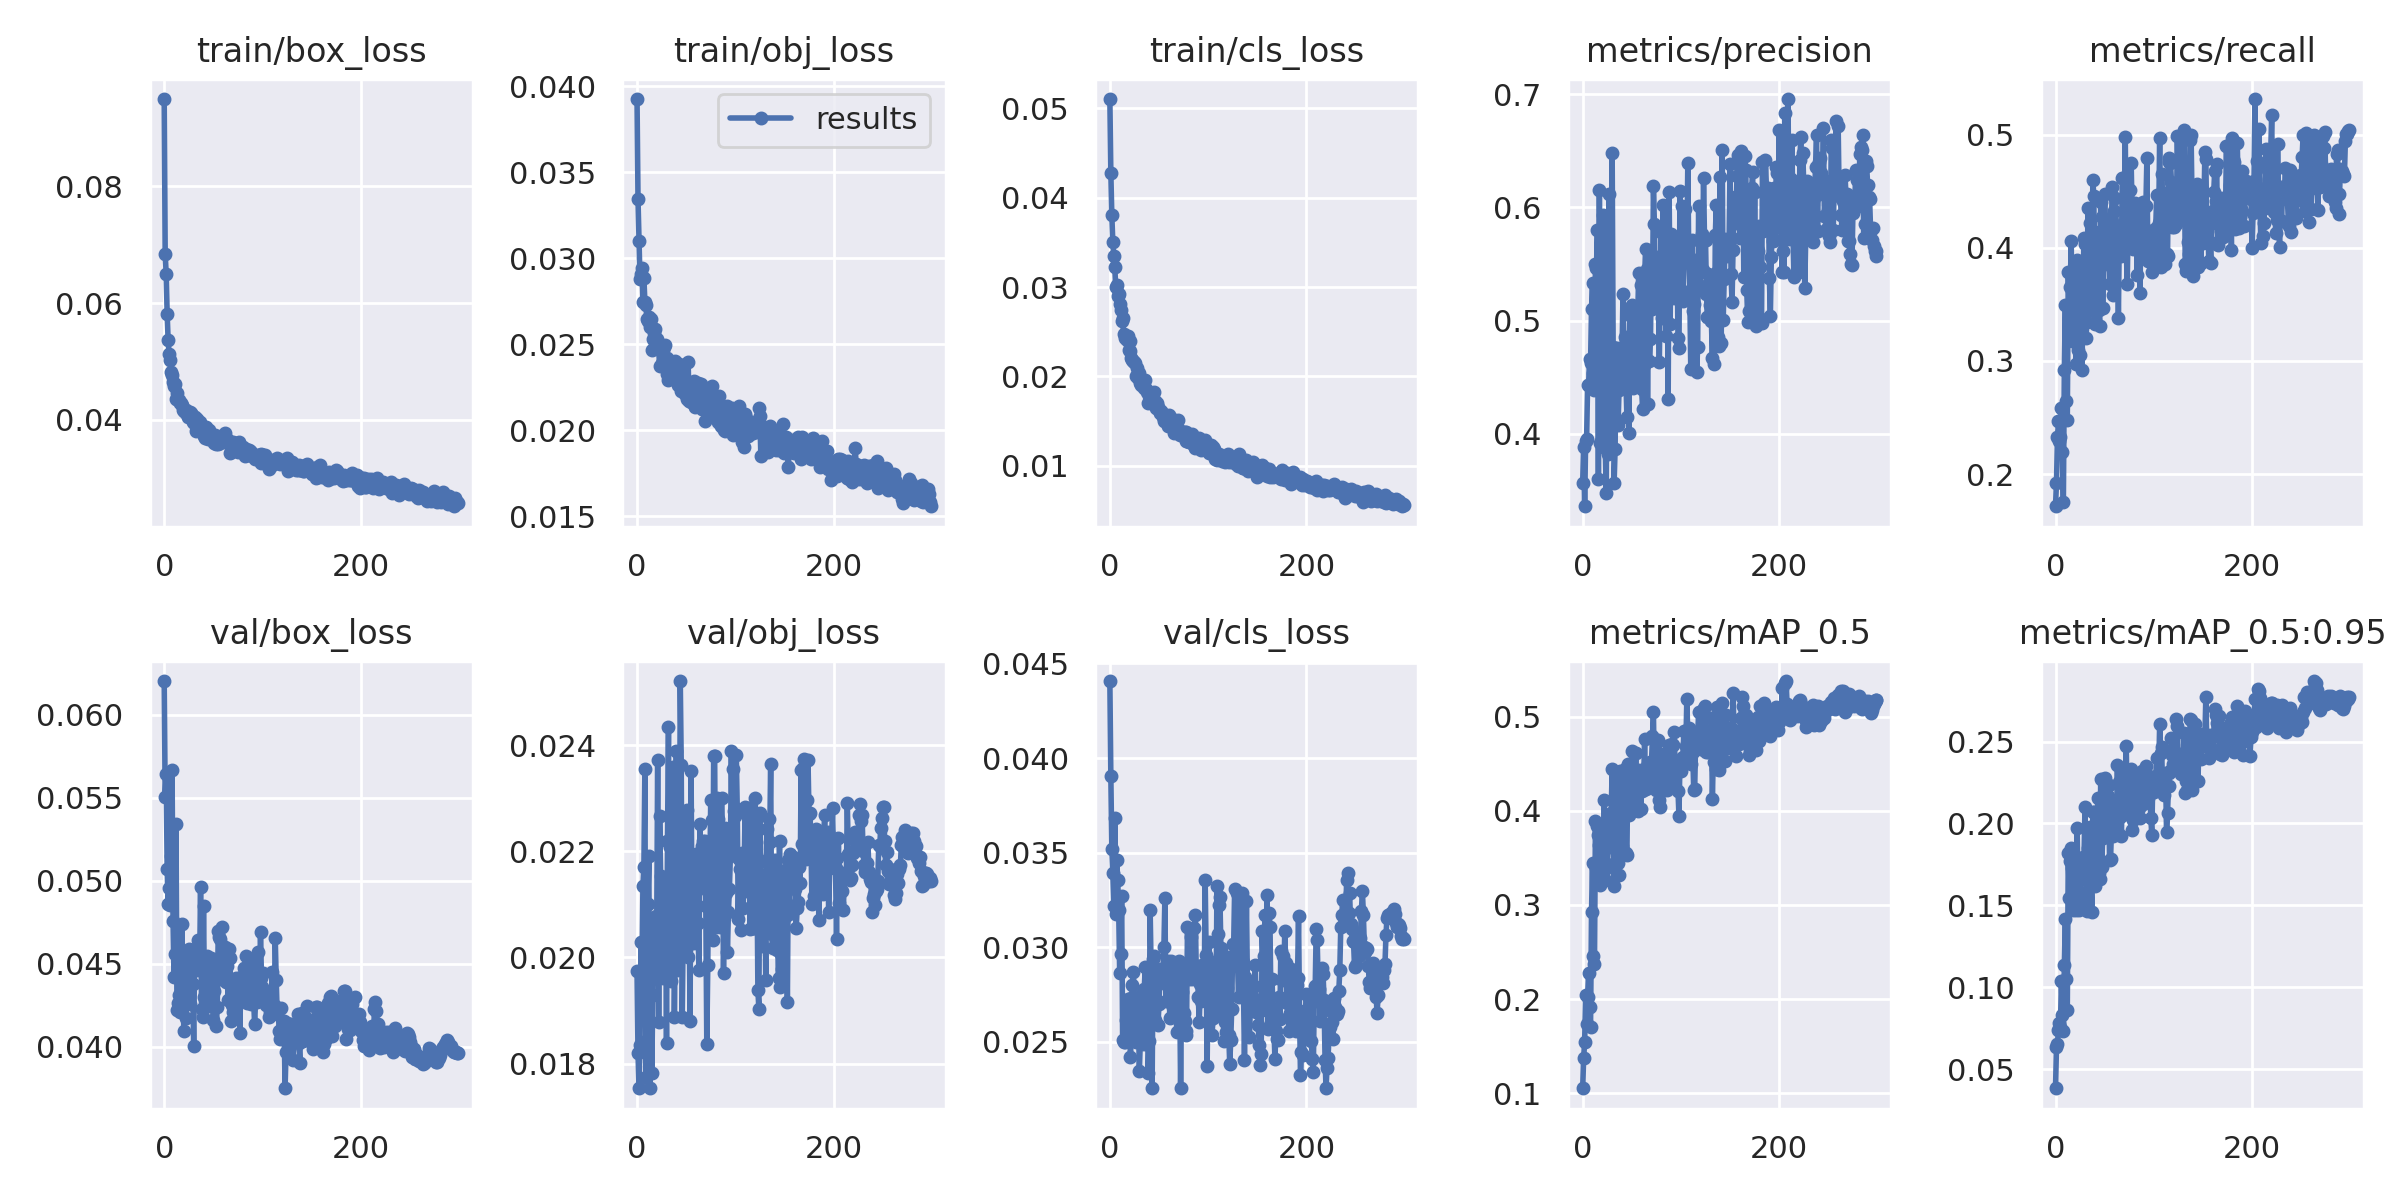
\includegraphics[width=\linewidth]{results.png}
	\caption{Statistics of the prototype training}
	\label{fig:res}
\end{figure}

\newpage
The precision is expected to increase however in the results displayed the opposite. This is not desirable as it means that the model is getting less precise as training goes on. Although, the model that will be used is the best performing one.

\newpage
\section{Hazy Command Line Help}

\begin{figure}[h!]
	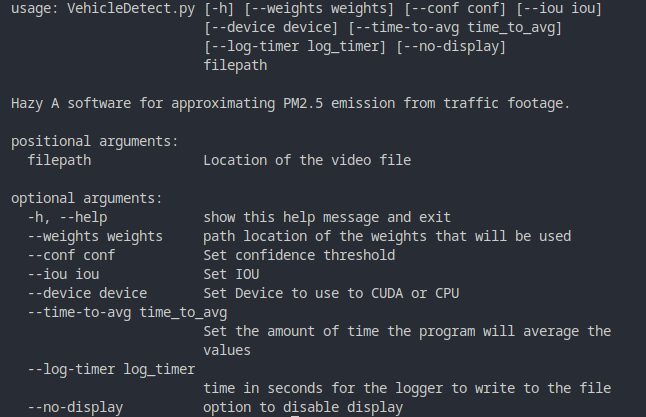
\includegraphics[width=\linewidth]{cmd_help.png}
	\caption{Hazy command line help shown}
	\label{fig:cmdhelp}
\end{figure}




Figure \ref{fig:cmdhelp} shows the command line help for the “VehicleDetect” program. This helps the user to determine what the different arguments do and what is needed to run the program. This can be accessed via the terminal by inputting the command “python VehicleDetect.py -–help” or “python VehicleDetect.py -h”.

\section{Object Detection}

The trained weights obtained by training were used in pre-recorded videos to determine if the weights were trained successfully and to see how they perform in actual video footage.  Figures \ref{fig:StreetView} and \ref{fig:BirdsEye} are screenshots of video recordings taken at Luna St., Lapaz and Diversion Road, Mandurriao, Iloilo City, Iloilo, Philippines , respectively. These recordings were then processed using the custom vehicle detection python file. The processing includes detecting the vehicles, drawing bounding boxes, and calculating and displaying the approximation of the emission of that area. The “detect.py” file that comes with yolov5 will not be used because it is an all-purpose detection algorithm and it cannot do the calculations needed for the project whereas the custom vehicle detection file has the sole purpose of calculating the emissions.

The trained model correctly identifies several vehicles on the road as shown enclosed in bounding boxes with the class name and confidence score above them.


\begin{figure}[h!]
	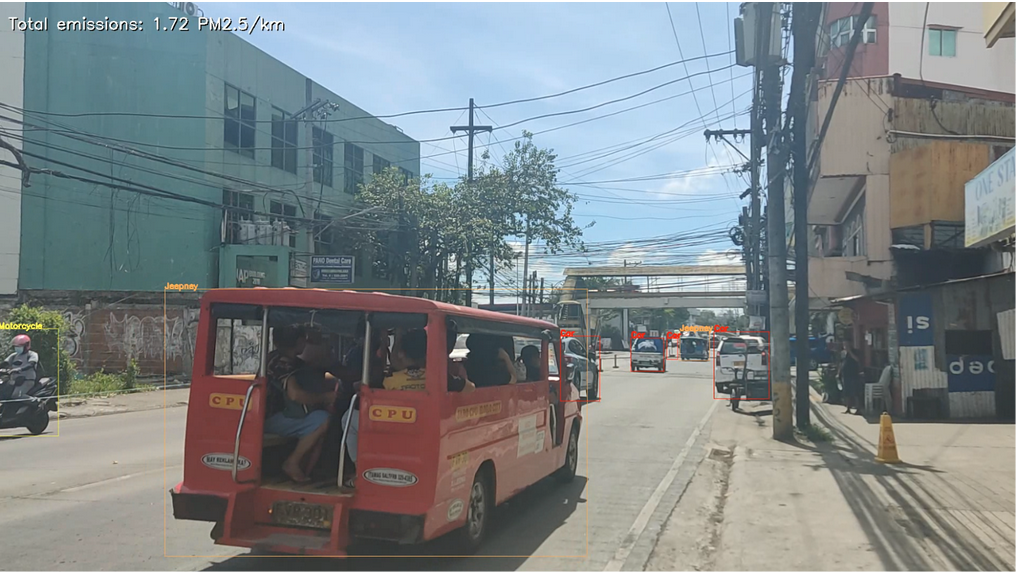
\includegraphics[width=\linewidth]{StreetView.png}
	\caption{Object Detection Prototype used for Traffic recorded in street view}
	\label{fig:StreetView}
\end{figure}

\begin{figure}[h!]
	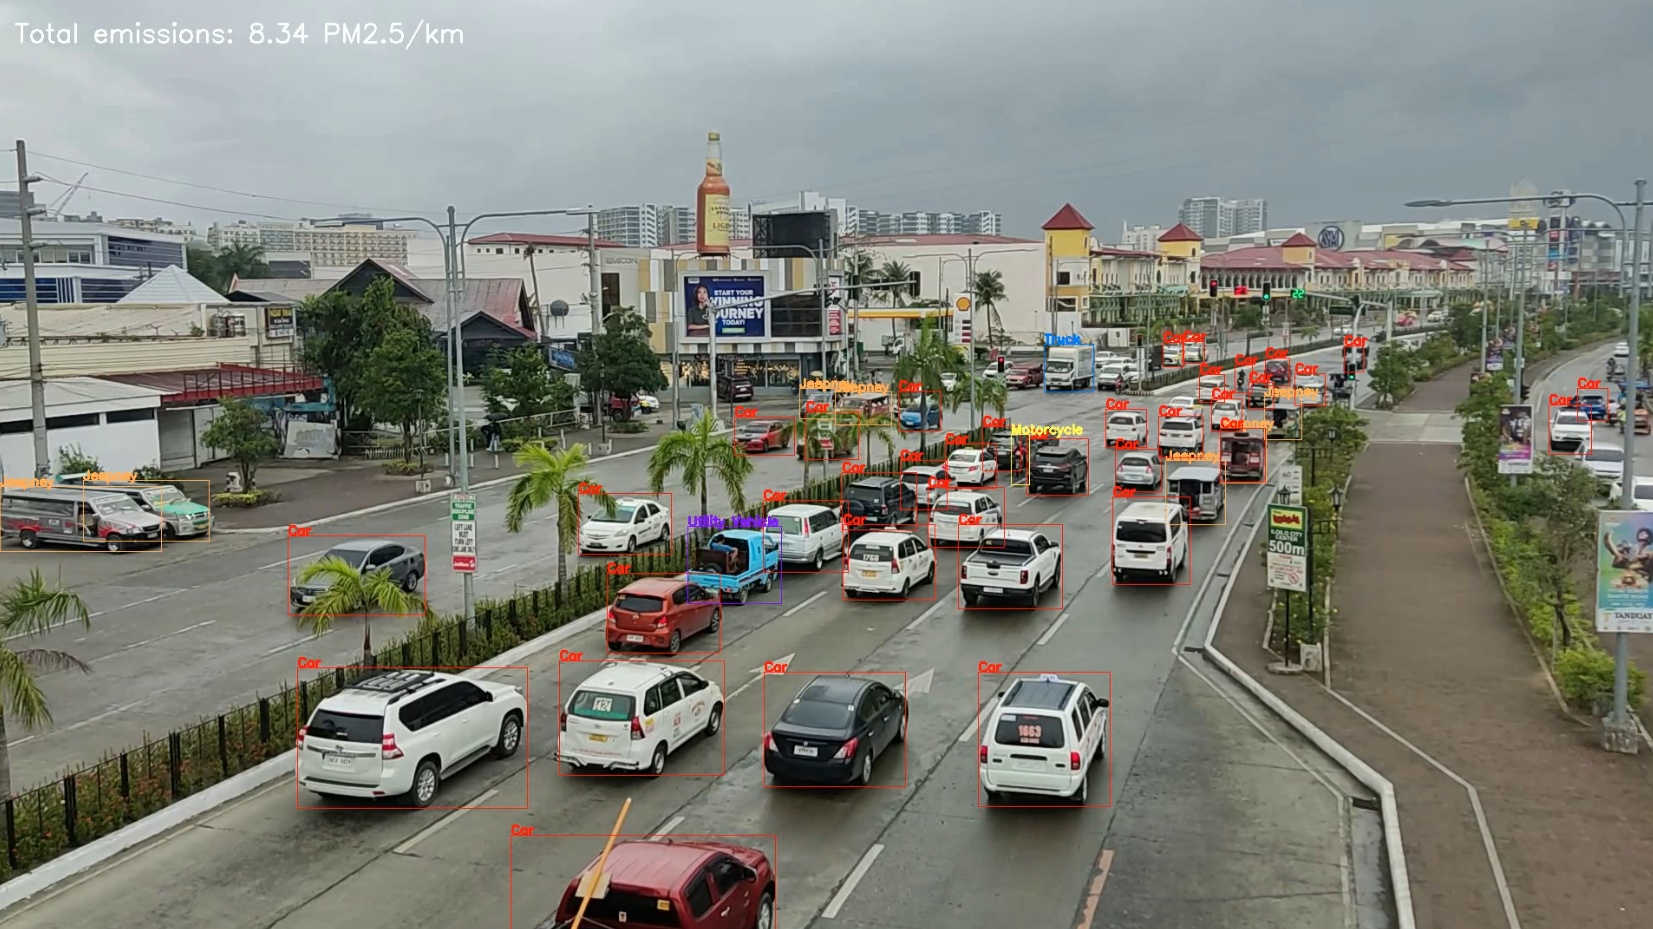
\includegraphics[width=\linewidth]{BirdsEye.png}
	\caption{Object Detection Prototype used for Traffic recorded in bird's eye view}
	\label{fig:BirdsEye}
\end{figure}

\newpage
The researchers compared the frame of the detected vehicle (Figure \ref{fig:BirdsEye}) from manual vehicle counting and below are the results:

\begin{table}[ht]   %t means place on top, replace with b if you want to place at the bottom
	\centering
	\caption{Comparison of manual counting versus detection from Figure \ref{fig:BirdsEye}} \vspace{0.25em}
	\begin{tabular}{|c|c|c|c|c|} \hline
		\centering  & 	\multicolumn{2}{|c|}{\textbf {Actual}} & 	\multicolumn{2}{|c|}{\textbf {Detected}} \\ \hline
		\textbf {Vehicle type} & Count & Total $PM_{2.5}$  & Count & Total $PM_{2.5}$ \\ \hline
		Tricycle   & 3  & 0.1686 & 0 & 0\\ \hline
		Motorcycle& 3  &0.1008  & 1 & 0.0336\\ \hline
		Jeepney &7 &5.9262  &6	& 5.0796\\ \hline
		Car & 46 & 1.0166  & 36  & 0.7956\\ \hline
		Utility Vehicle & 3 & 0.429 & 1 & 0.143\\ \hline
		Truck & 2 & 1.5038 & 1 & 0.7519\\ \hline
		
		\textbf{Average $PM_{2.5}$} & & 9.145 & & 6.8037\\ \hline
		
	\end{tabular}
	\label{tab:emission}
\end{table}


There is a difference in the number of vehicles in the detection and manual counting and this might be due to low detail on some vehicles, for example on the upper right corner of Figure \ref{fig:StreetView} there are several vehicles, like the three tricycles, that are not detected by the program, or obstruction of objects, like on the case of one truck that is obstructed by the tree on the upper left corner of Figure \ref{fig:StreetView}. The actual value of PM2.5 using manual counting is 9.145 while the detection only shows 6.8037.

\newpage
\section{Log File}
\begin{figure}[h!]
	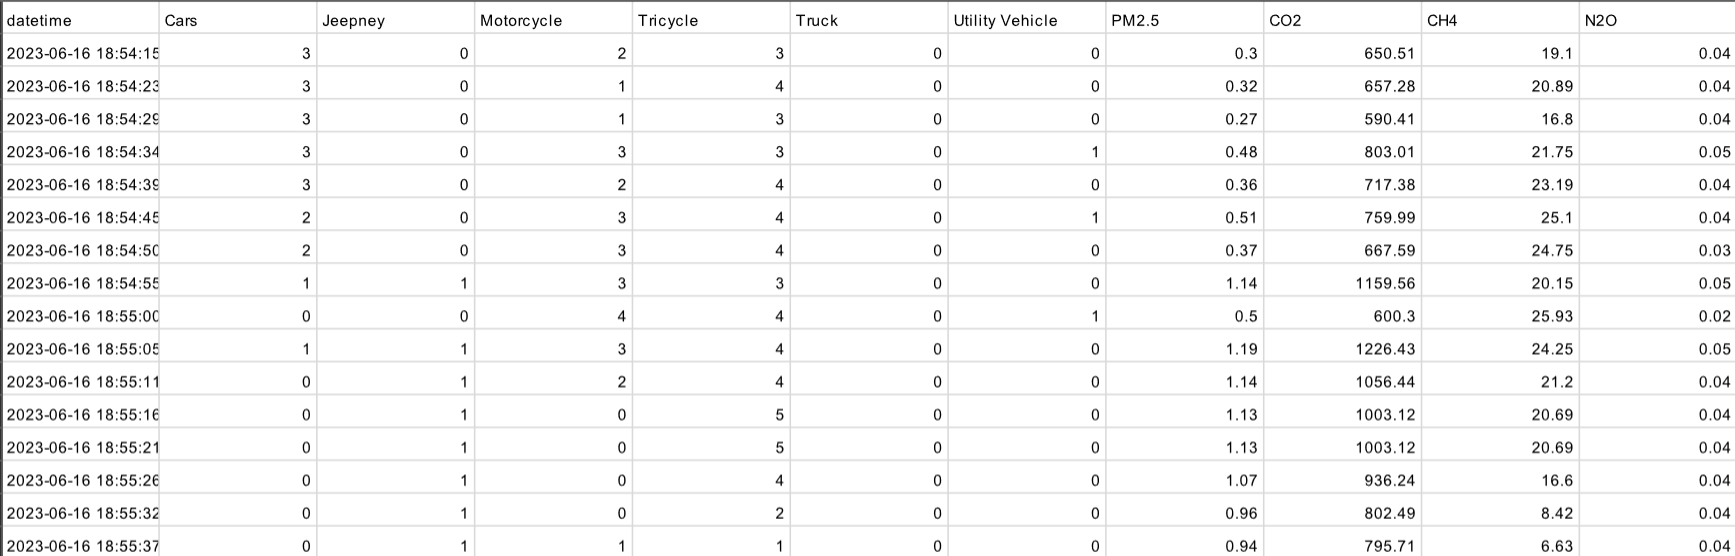
\includegraphics[width=\linewidth]{logfile.png}
	\caption{Example Logfile where each entry was generated for approximately 5 seconds}
	\label{fig:logfile}
\end{figure}

To record the data, the results were saved in a CSV file as shown in Figure \ref{fig:logfile}. The recorded data was written using the current frame that it was recorded in, not the average, hence why the values on the recorded data vary a lot between time periods. The data in Figure \ref{fig:logfile} shows that Cars have the most contribution to particle emissions with an average of 17.7 cars per recording, followed by the jeepney having an average of 8.4 jeepneys per recording. Tricycles and Utility Vehicles came last with almost none of them per recording.




